\documentclass{article}

\bibliographystyle{plain}

\usepackage{epsfig}
\usepackage{xcolor}
\usepackage{float}
\usepackage{amsmath}
\usepackage{amssymb}
\usepackage[export]{adjustbox}
\usepackage{afterpage}
\usepackage{caption}
\usepackage{subcaption}
\usepackage{graphicx} % Required for inserting images

\begin{document}

\title{Performance Improvement of Chombo 4}
\author{Simon Zhang}
\date{September 2023}

\maketitle

\section{Introduction}
To improve the performance of Chombo 4, we ran weak scaling tests and manipulated inputs on the EBINS example in Chombo 4.

\section{Methodology}
\subsection{Weak Scaling Test}
\subsubsection{CPU}
To determine the performance bottlenecks of Chombo 4, weak scaling tests were run on NERSC Perlmutter CPU nodes using cray-mpich and mpich modules. We started the tests using 1 core of 1 CPU node in the domain of $nx = 32$ and maximum grid of $64$ for mpich module. From there, we increased the number of processors/core by $1.5^3$ and the domain ($nx$) by $1.5$ until the processors ran out of memory, which is $12$ processors with a domain of 72. Meanwhile, weak scaling tests were conducted using cray-mpich module starting from 1 core of 1 CPU node in the domain of $nx=32$ and maximum grid of $64$ increasing to the domain of $nx=64$ and $nx=96$, under the same increments for mpich module.

Weak scaling tests were also run on NERSC Perlmutter CPU nodes by using different number of processors and size of domain. We started the tests using 1 core of 1 CPU node in the domain of $nx = 32$ and maximum grid of $32$. From there, we increased the number of processors/core by $2^3$ and the domain ($nx$) by $2$ until the processors ran out of memory, which is $27$ processors with a domain of $96$. By doing so, Chombo 4 is handling problems with the size of 1 box, 8 boxes, and 27 boxes such that we are using the same number of processors to handle the same number of boxes.

\subsubsection{GPU}
Weak scaling tests were run on NERSC Perlmutter GPU nodes. We started the tests using 1 GPU of 1 GPU node in the domain of $nx=32$ and maximum grid of $32$. From there, we increased the number of GPUs to $8$ to handle a domain of $nx=64$ since we would get 8 boxes for this domain. However, the GPU nodes ran out of memory as we try to increase domain to $nx=96$ for $27$ GPUs due to GPU nodes having less total aggregate memory than the CPU nodes.

\subsection{W Cycle}
To improve the performance improvement of Chombo 4, we decided to manipulate $num$\_$smooth$ and $use$\_$w$\_$cycle$. $num$\_$smooth$ controls the number of times the initial system is iterated or relaxed until residual is a smooth function and $use$\_$w$\_$cycle$ controls whether w-cycle: a multigrid method, is turned on or off. 
Specifically, jobs were ran with CPU processors and GPUs under the same increment pattern as weak scaling tests, where $nx$ increase by 2, processors and GPUs increase by $2^3$ with the maximum grid of $32$. Additionally, $num$\_$smooth$ started from $2$ to $8$ increasing by a factor of 2 and $use$\_$w$\_$cycle$ is equated to true or false.

\section{Findings}
\subsection{Weak Scaling Test}
\subsubsection{CPU}

We find that runs loaded with mpich module scale better on the CPU Nodes as we increase the processor count and domain (Figure \ref{fig:mpich vs cray-mpich}).

\begin{figure}[ht]
\centering
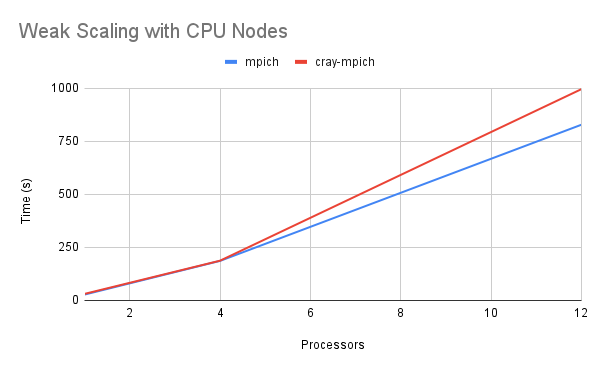
\includegraphics[width=12cm]{Weak Scaling with CPU Nodes (1.5x).png}
\caption{Weak Scaling of CPU Nodes using mpich and cray-mpich modules}
\label{fig:mpich vs cray-mpich}
\end{figure}

\subsection{W Cycle}
We find that using $num$\_$smooth$ = 16 without w Cycle scales the best (Figure \ref{fig:CPU nodes with and without w cycle}) while any combination of $num$\_$smooth$ and $use$\_$w$\_$cycle$ does not affect the scaling of Chombo 4 significantly (Figure \ref{fig:GPU nodes with and without w cycle}). 

\begin{figure}[H]
        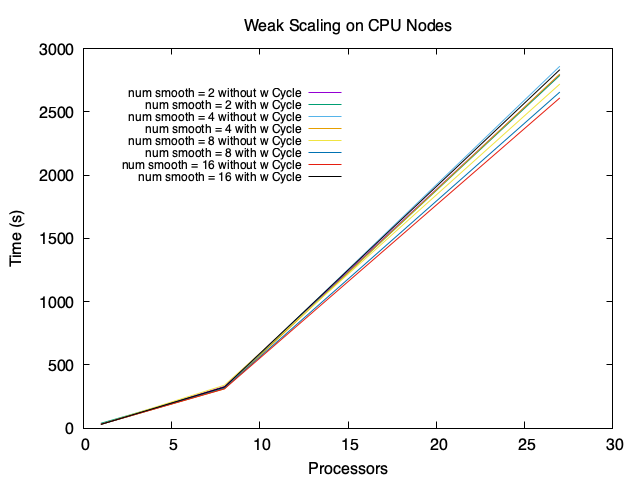
\includegraphics[width=\textwidth]{Weak Scaling on CPU Nodes.png}
        \caption{Weak Scaling Tests of CPU Nodes with and without w Cycle}  
        \label{fig:CPU nodes with and without w cycle}
\end{figure}
\begin{figure}[H]
        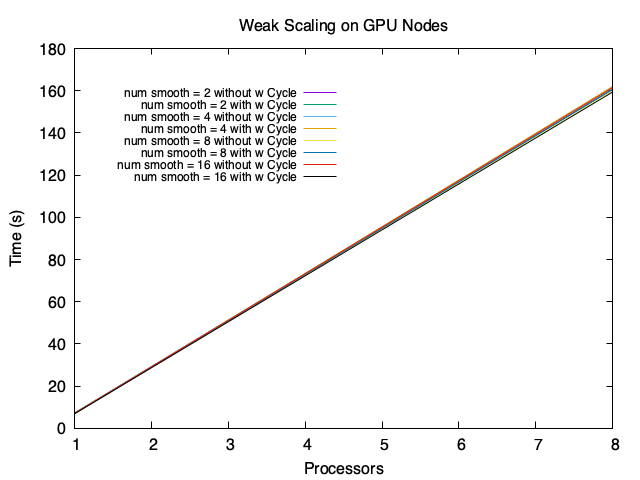
\includegraphics[width=\textwidth]{Weak Scaling on GPU Nodes.png}
        \caption{Weak Scaling Tests of GPU Nodes with and without w Cycle}  
        \label{fig:GPU nodes with and without w cycle}
\end{figure}

We find that different processors/GPUs have different optimal $num$\_$smooth$ in terms of runtimes (Figure \ref{fig:Performance on CPU Nodes}, \ref{fig:Performance on GPU Nodes}).

\begin{figure}[H]
    \begin{subfigure}{0.92\textwidth}
        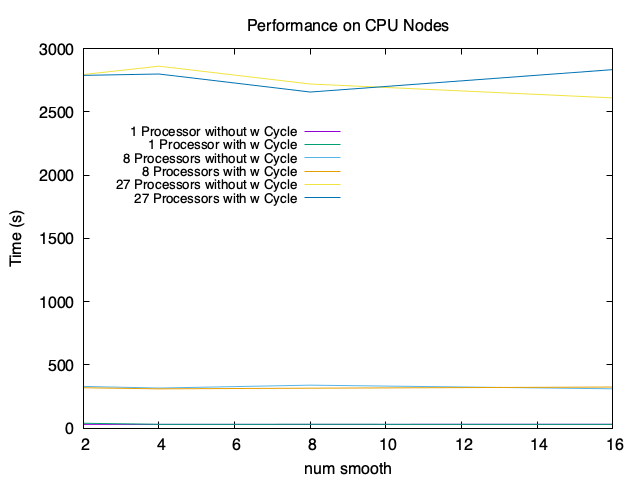
\includegraphics[width=\textwidth]{Performance on CPU Nodes.png}
        \caption{CPU Processors}
        \label{fig:Performance on CPU Nodes}
    \end{subfigure}
    \begin{subfigure}[b]{0.92\textwidth}
        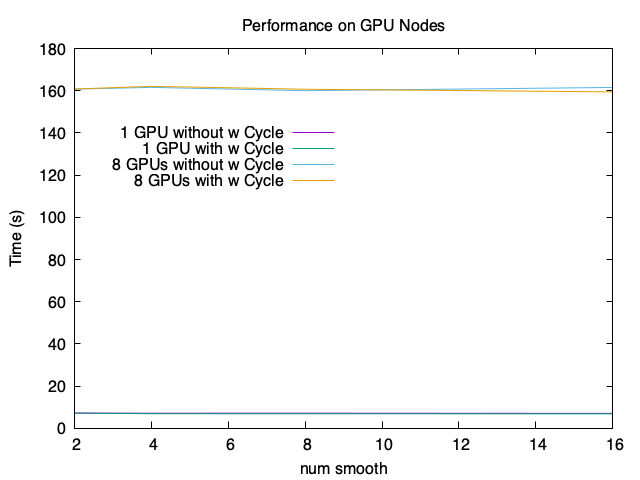
\includegraphics[width=\textwidth]{Performance on GPU Nodes.png}
        \caption{GPUs}
        \label{fig:Performance on GPU Nodes}
    \end{subfigure}
    \caption{Performance of CPU Processors and GPUs under various $num$\_$smooth$}
\end{figure}

\end{document}
